\documentclass[11pt]{article}
\usepackage[utf8]{inputenc}
\usepackage[a4paper,margin=1in]{geometry}
\usepackage{hyperref,enumitem,titlesec,xcolor,fancyhdr,tikz,graphicx,eso-pic}
\graphicspath{{../}}
\definecolor{kcpc-text}{RGB}{20,20,20}
\definecolor{kcpc-muted}{RGB}{90,90,90}
\definecolor{kcpc-red}{RGB}{176,0,0}
\pagestyle{fancy}\fancyhf{}
\lhead{\textcolor{kcpc-text}{\small\bfseries Papers}}
\rhead{\textcolor{kcpc-muted}{\small Week 5}}
\cfoot{\textcolor{kcpc-muted}{\small KCPC}}
\renewcommand{\headrulewidth}{0.4pt}
\renewcommand{\headrule}{\hbox to\headwidth{\color{kcpc-red}\leaders\hrule height \headrulewidth\hfill}}
\renewcommand{\footrulewidth}{0pt}
\setlength{\headheight}{28pt}
\AddToShipoutPictureBG{\begin{tikzpicture}[remember picture,overlay]
  \node[opacity=0.035,at=(current page.center)]{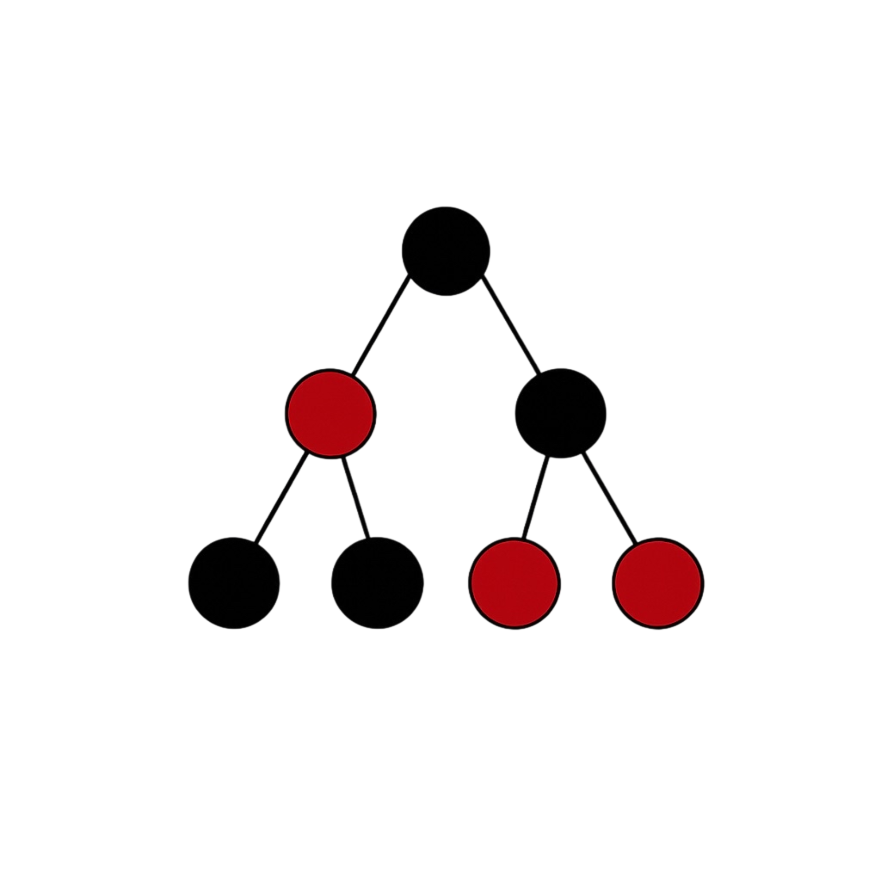
\includegraphics[width=0.38\paperwidth]{kcpc-logo.png}};
\end{tikzpicture}}
\titleformat{\section}{\large\bfseries\color{kcpc-red}}{}{0pt}{}
\titleformat{\subsection}{\normalsize\bfseries}{\thesubsection}{1em}{}
\setlist[itemize]{noitemsep,topsep=4pt}
\hypersetup{colorlinks=true,urlcolor=kcpc-red,linkcolor=kcpc-red}
\title{KCPC Week 5 Papers\\Graphs II: Dijkstra and 0--1 BFS}
\author{King's Competitive Programming Club}
\date{}

\begin{document}
\maketitle\thispagestyle{fancy}

An annotated guide to the original research behind Workshop 5, which introduces shortest-path algorithms in weighted graphs --- Dijkstra's algorithm and 0--1 BFS --- and situates them in their broader theoretical and historical context. Each entry gives a complete citation, a stable location and the part relevant to the slides and exercises. For a gentler first pass, use \emph{Week 5 Reading}; these are primary sources, not introductory tutorials.

\section*{I. Foundational papers}

\subsection*{[1] Dijkstra, E. W. (1959)}
\textit{A note on two problems in connexion with graphs.}
Numerische Mathematik, 1, 269--271.
\url{https://doi.org/10.1007/BF01386390}

\textbf{Where / why:} The whole note is three pages; the shortest-path development is ``problem 2'', pp.~269--271. This introduces Dijkstra's algorithm, the primary shortest-path method taught in the workshop for graphs with non-negative edge weights, and the source of the slides' settling invariant.

\subsection*{[2] Moore, E. F. (1959)}
\textit{The shortest path through a maze.}
Proceedings of the International Symposium on the Theory of Switching, Harvard University Press, 285--292.

\textbf{Where / why:} Establishes breadth-first search as a shortest-path method in unweighted graphs, forming the conceptual foundation for both Dijkstra's algorithm and 0--1 BFS (slides: graph foundations and multi-source BFS).

\subsection*{[3] Lee, C. Y. (1961)}
\textit{An algorithm for path connections and its applications.}
IRE Transactions on Electronic Computers, EC-10(3), 346--365.
\url{https://doi.org/10.1109/TEC.1961.5219222}

\textbf{Where / why:} Demonstrates BFS-based shortest-path techniques in structured grid environments; the historical root of the grid-as-implicit-graph modelling used throughout the problem sheet.

\section*{II. Structural and data-structure improvements}

\subsection*{[4] Dial, R. B. (1969)}
\textit{Algorithm 360: Shortest-path forest with topological ordering.}
Communications of the ACM, 12(11), 632--633.
\url{https://doi.org/10.1145/363269.363610}

\textbf{Where / why:} The full note, pp.~632--633, introduces bucket-based shortest-path methods for small integer weights, providing the theoretical basis for the 0--1 BFS optimisation (slides: two adjacent distance levels).

\subsection*{[5] Fredman, M. L., \& Tarjan, R. E. (1984)}
\textit{Fibonacci heaps and their uses in improved network optimization algorithms.}
Journal of the ACM, 34(3), 596--615.
\url{https://doi.org/10.1145/28869.28874}

\textbf{Where / why:} Introduces the Fibonacci heap; the network-optimisation applications give Dijkstra's algorithm its textbook $O(m+n\log n)$ bound. This shows how priority queue design impacts the efficiency of Dijkstra's algorithm; our workshops use the simpler lazy binary heap.

\subsection*{[6] Johnson, D. B. (1977)}
\textit{Efficient algorithms for shortest paths in sparse networks.}
Journal of the ACM, 24(1), 1--13.
\url{https://doi.org/10.1145/321992.321993}

\textbf{Where / why:} Demonstrates extensions and optimisations of Dijkstra's algorithm for sparse graphs, the regime in which competitive programming problems almost always live.

\section*{III. Advanced and modern developments}

\subsection*{[7] Thorup, M. (1999)}
\textit{Undirected single-source shortest paths with positive integer weights in linear time.}
Journal of the ACM, 46(3), 362--394.
\url{https://doi.org/10.1145/316542.316548}

\textbf{Where / why:} Proves that single-source shortest paths can be solved in linear time under restricted (undirected, positive integer) weight conditions, bypassing comparison-based priority queues entirely.

\subsection*{[8] Duan, R., Mao, J., Mao, X., Shu, X., \& Yin, L. (2025)}
\textit{Breaking the sorting barrier for directed single-source shortest paths.}
Proceedings of the 57th Annual ACM Symposium on Theory of Computing (STOC 2025), 36--44.
\url{https://doi.org/10.1145/3717823.3718179} (also arXiv:2504.17033)

\textbf{Where / why:} Gives a deterministic $O(m\log^{2/3} n)$-time directed SSSP algorithm, the first to break Dijkstra's $O(m+n\log n)$ bound on sparse graphs when only distances (not their ordering) are required.

\subsection*{[9] Duan, R., Mao, X., Shu, X., \& Yin, L. (2026)}
\textit{A faster directed single-source shortest path algorithm.}
arXiv:2602.07868.
\url{https://arxiv.org/abs/2602.07868}

\textbf{Where / why:} Sharpens [8] to $O(m\sqrt{\log n}+\sqrt{mn\log n\log\log n})$. Included to show that single-source shortest paths remain an active theoretical topic: even classical problems continue to admit structural improvements under refined models.

\section*{Summary}
Together, these papers trace the development of single-source shortest-path algorithms: from the original formulations of BFS and Dijkstra's method [1--3], through bucket, heap and sparse-graph optimisations [4--6], to linear-time integer methods and the recent directed-graph breakthroughs [7--9]. They situate the techniques presented in this workshop within their broader theoretical lineage. For implementation-level expositions with page references, see \emph{Week 5 Reading}.

\end{document}
